\section{Test}
\subsection{Test Acceso}
\subsubsection{Diagrama de flujo}
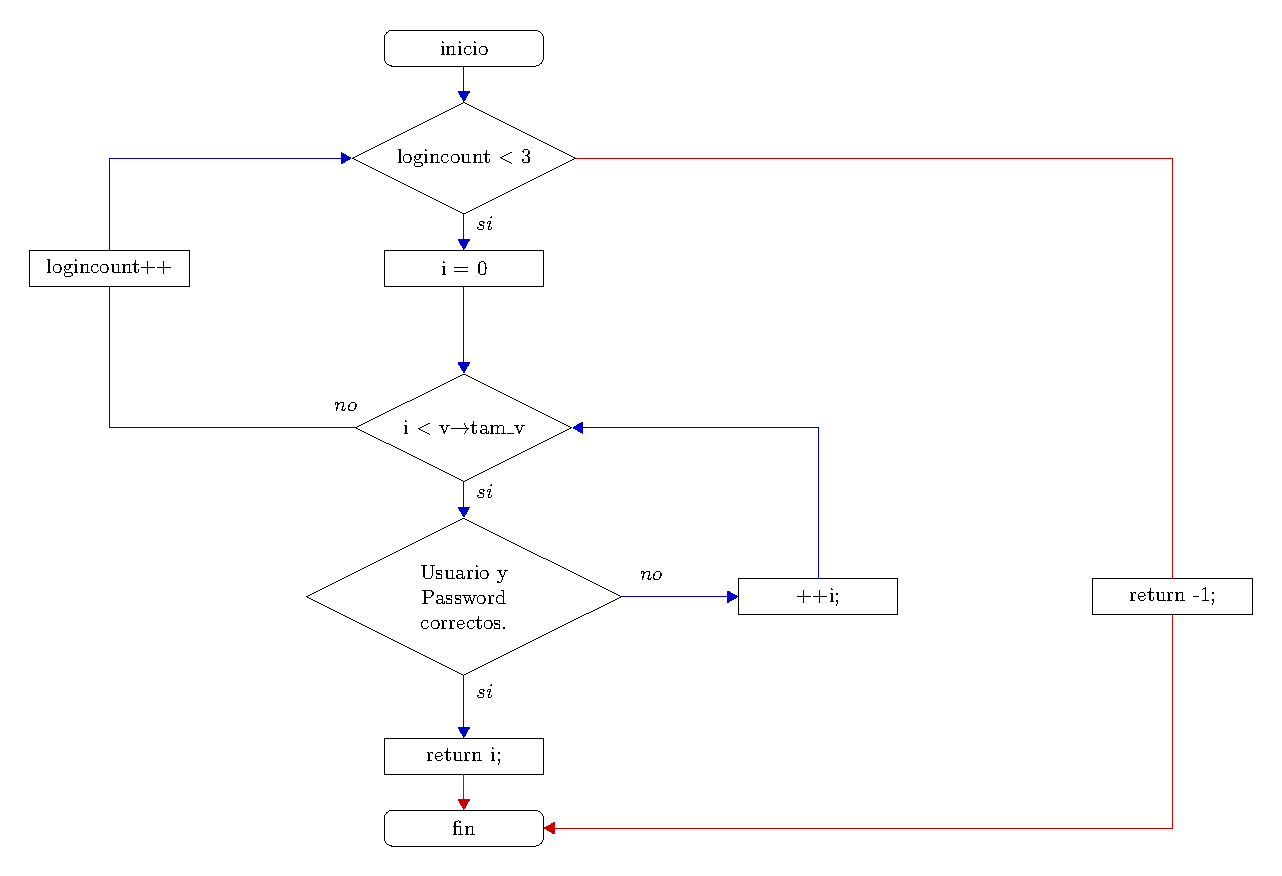
\includegraphics[width=\textwidth, angle=0,scale=0.75]{dep/flujoacceso.pdf}
\subsubsection{Complejidad Ciclomática}
\begin{itemize}
\item La complejidad ciclomática de esta función es --> V(G) = NA-NN+2 = 12-10+2 = 4
\end{itemize}
\subsection{Test Usuarios}
\subsubsection{Diagrama de flujo}
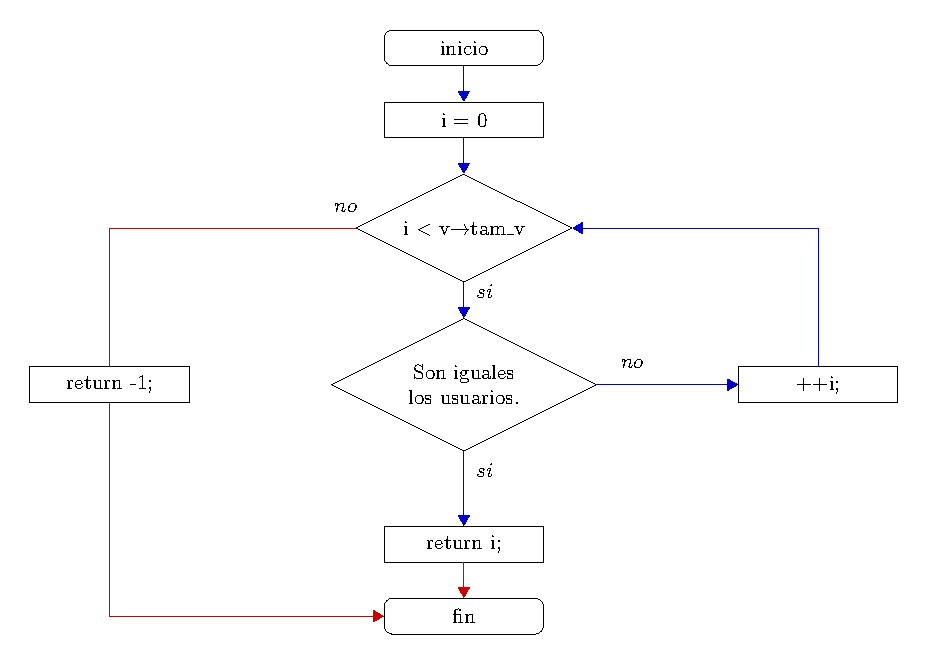
\includegraphics[width=\textwidth, angle=0,scale=0.75]{dep/flujousuarios.pdf}
\subsubsection{Complejidad Ciclomática}
\begin{itemize}
\item La complejidad ciclomática de esta función es --> V(G) = NA-NN+2 = 9-8+2 = 3
\end{itemize}
\subsection{Test Viajes}
\subsubsection{Diagrama de flujo}
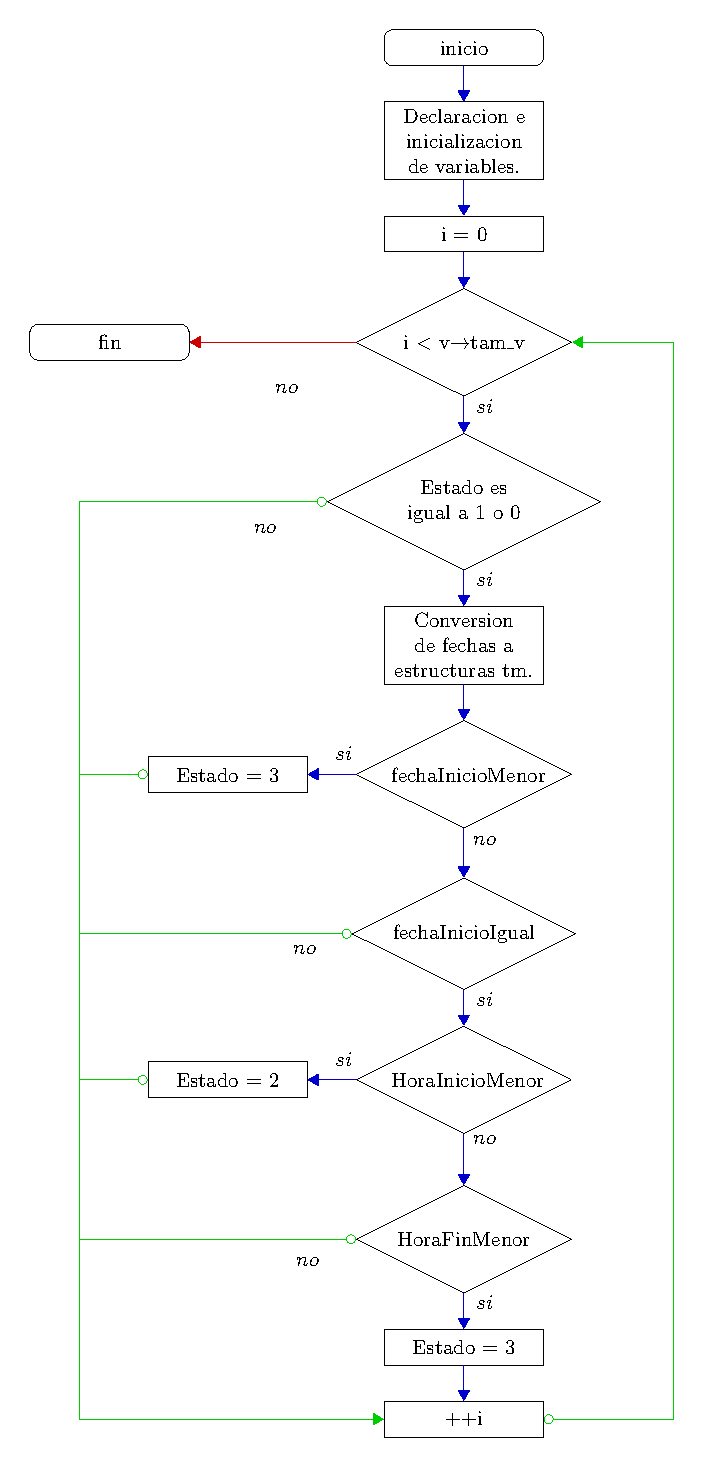
\includegraphics[width=\textwidth, angle=0,scale=0.68]{dep/flujoupviajes.pdf}
\subsubsection{Complejidad Ciclomática}
\begin{itemize}
\item La complejidad ciclomática de esta función es --> V(G) = NA-NN+2 = 20-15+2 = 7
\end{itemize}
\newpage
\subsection{Test Incidencias}
\subsubsection{Diagrama de flujo}
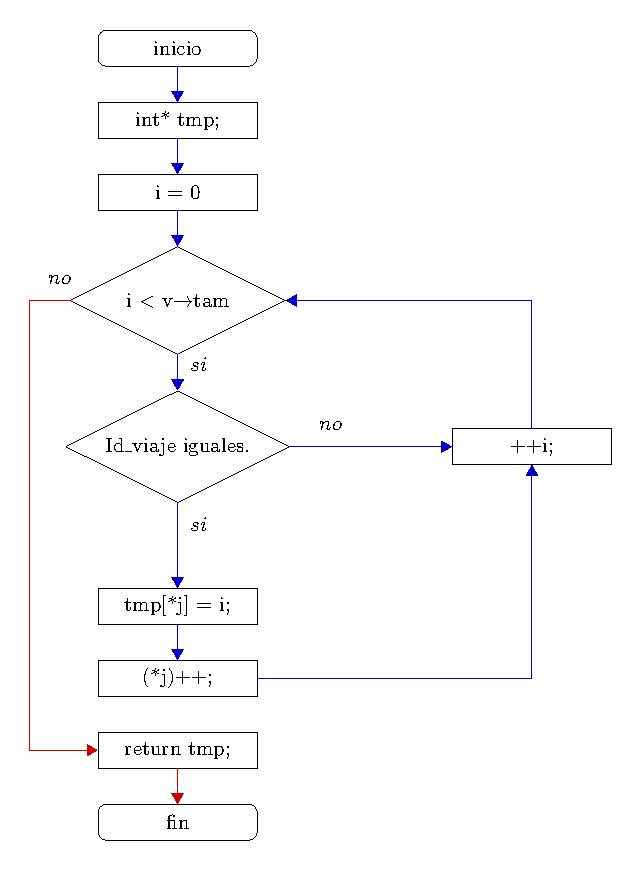
\includegraphics[width=\textwidth, angle=0,scale=0.75]{dep/flujolistaincidencia.pdf}
\subsubsection{Complejidad Ciclomática}
\begin{itemize}
\item La complejidad ciclomática de esta función es --> V(G) = NA-NN+2 = 11-10+2 = 3
\end{itemize}
